\chapter{Representación del sistema ROS2 con grafos de conexionado} \label{cap: anexo grafos nodos ros2}

El presente apéndice muestra el sistema de nodos de ROS2 con el que se ha trabajo en este proyecto. La representación se hace a través de un grafo de conexionado en el que se pueden apreciar los diferentes nodos partícipes y los sistemas de mensajes que emplean para comunicarse unos con otros.

\begin{landscape}
    \begin{figure}[h!]
    \centering
    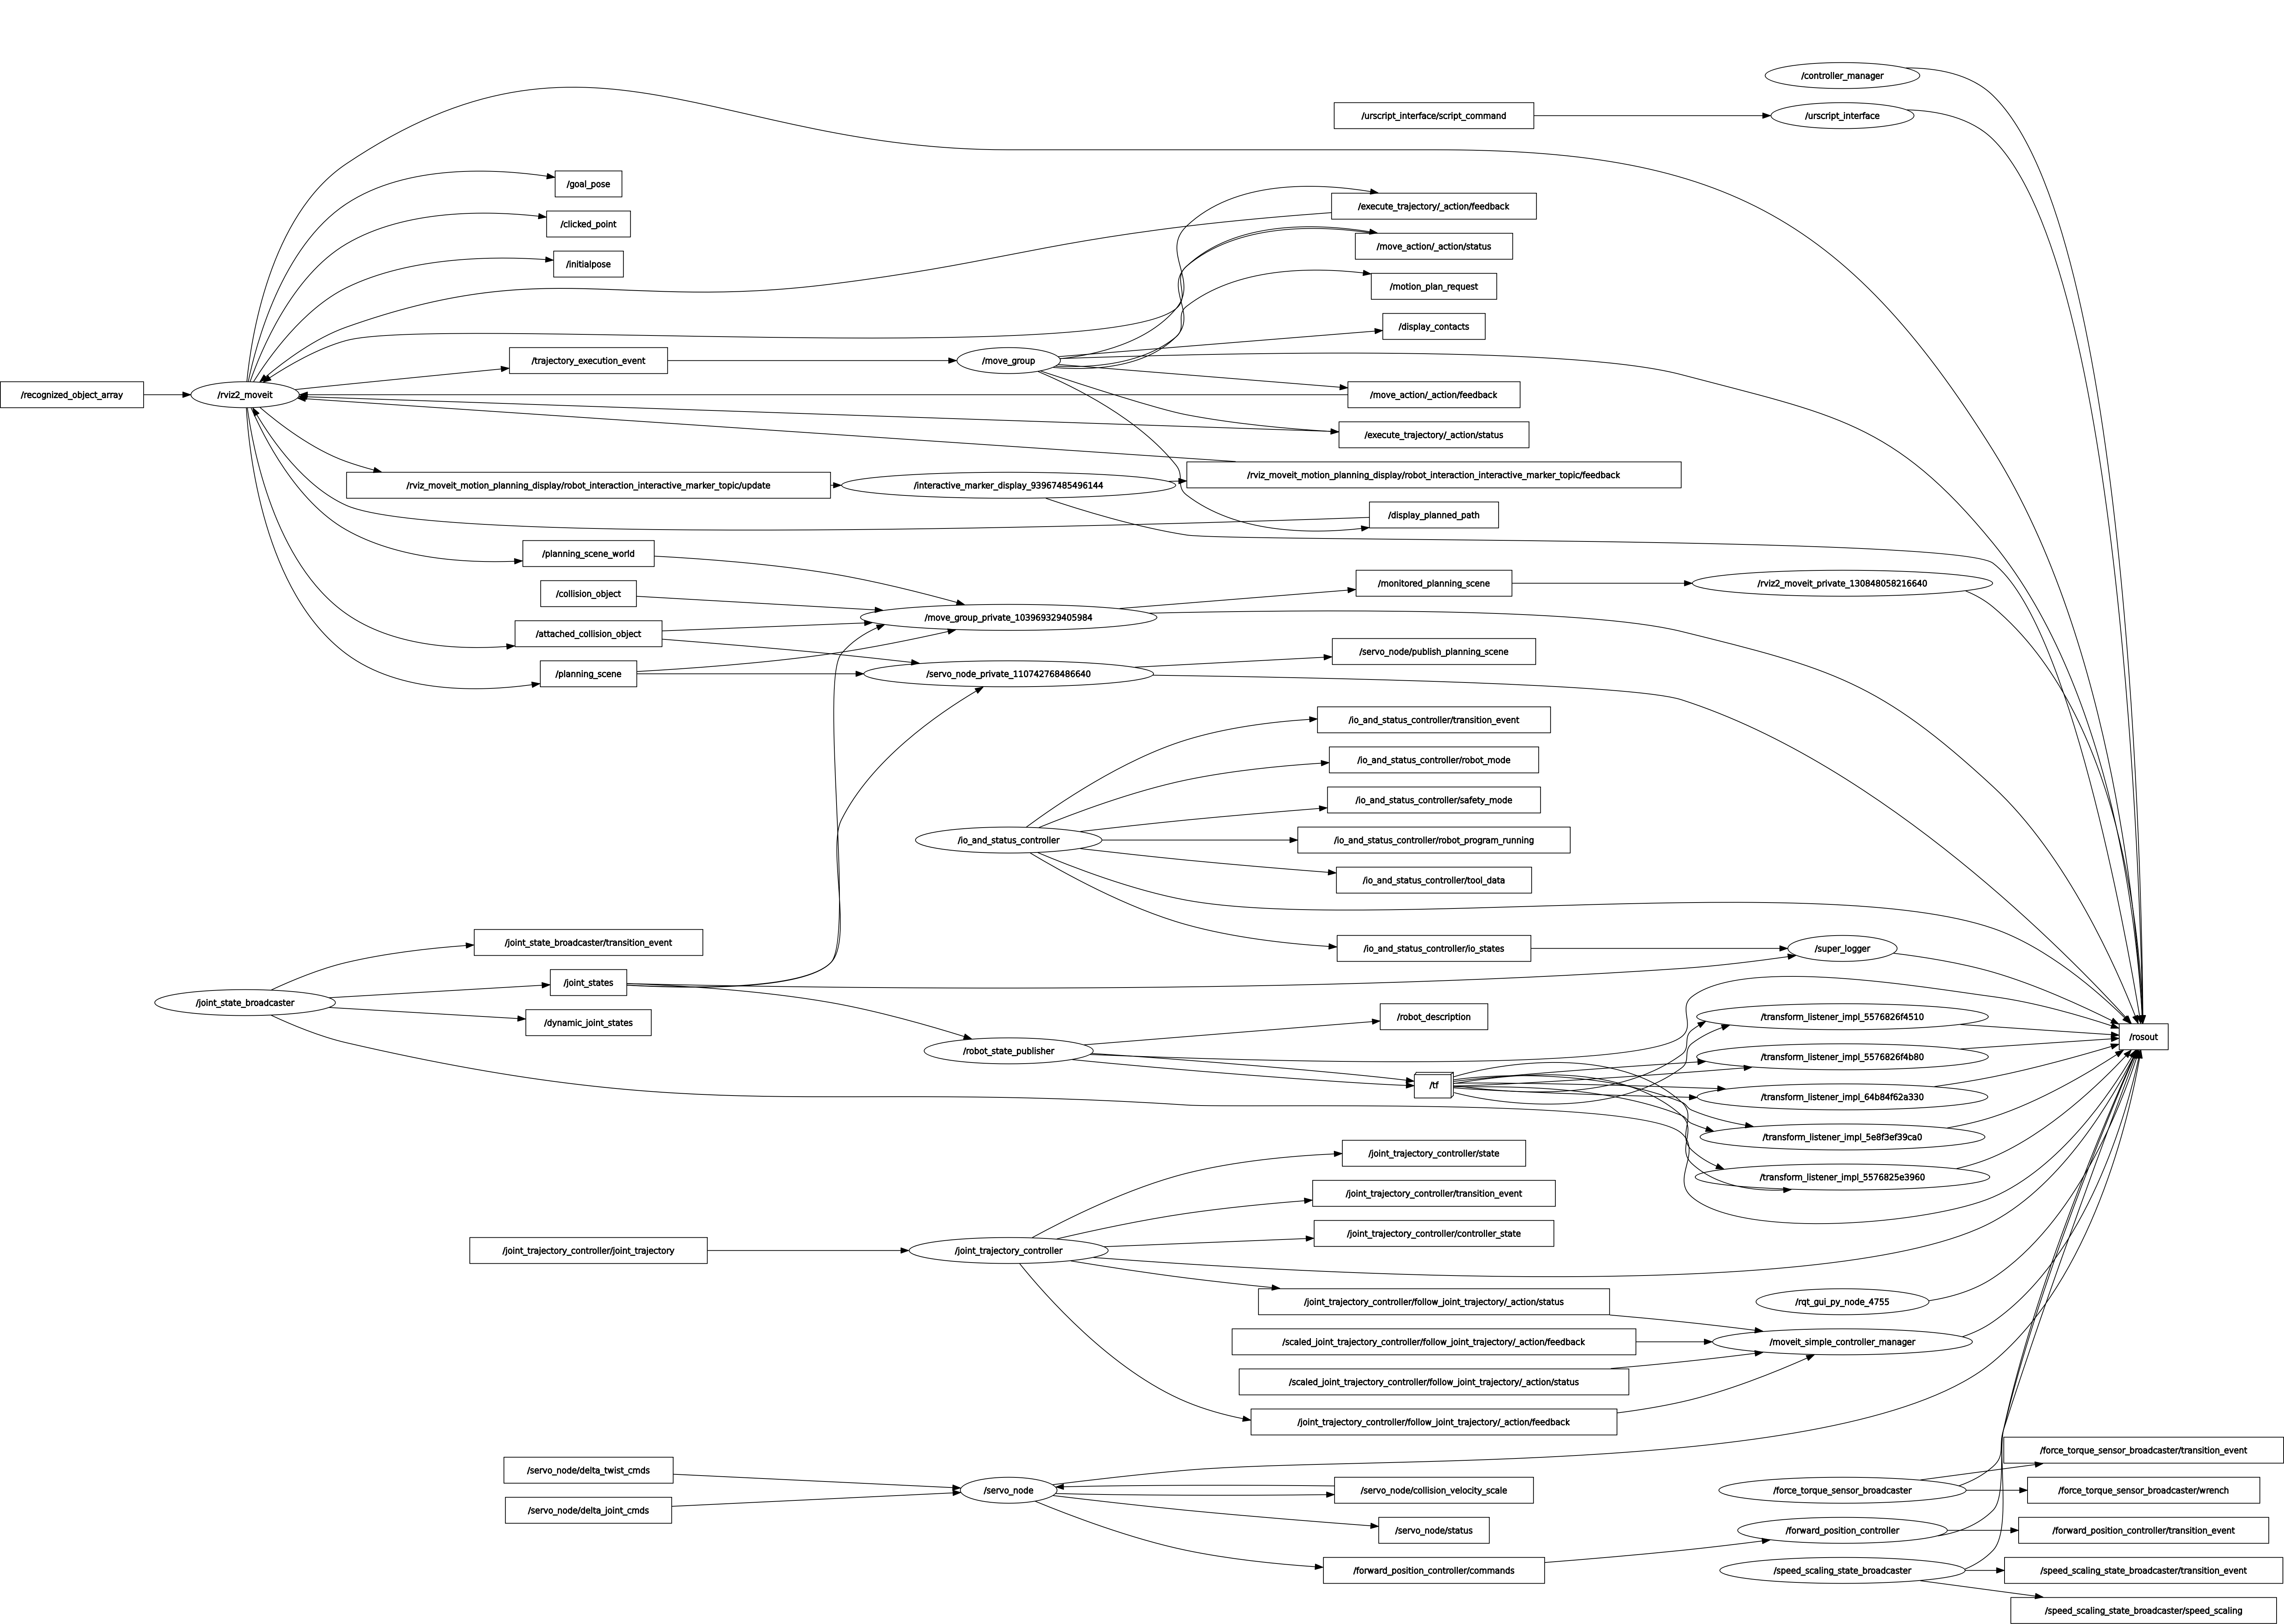
\includegraphics[scale=0.13, angle=0.0]{figuras/rosgraph super_logger.png}
    \caption{Grafo de conexionado de todo el entorno ROS2 empleado}
    \label{fig: grafo conexionado ros2}
\end{figure}
\end{landscape}

